\chapter{Chicago}\label{ch:ch2label}

Ce chapitre est exclusivement dédié au bidiplôme pour Chicago. C’est le bidiplôme le plus vaste, au moins 75\% des bidiplômes cités sur le site de l’ESEO ou de ce que l’on vous présente aux JPOS viennent d’ici. (Ce n’est pas 41 destinations différentes, mais bien 41 bidiplômes différents... nuancent)

\section{Les bidiplômes proposés}\label{sec:sec2.1}
Une multitude de bidiplômes est disponible pour Chicago et CE N'EST PAS QUE du management. C’est bien plus que cela: de l’électronique, de l’informatique, du biomédical, de l’électronique de puissance, etc. Vous avez un large panel de choix qui s’offrent à vous, ne vous arrêtez pas à l’idée reçue du management. \\
Je vous donne un lien général vers le site de l'IIT car il doit pas mal changer et à vrai dire je ne me souviens plus trop où est quoi... Je vous laisse donc chercher sur ce site et trouver les bonnes informations.\\
\href{https://admissions.iit.edu/graduate/apply/degree-seeking-checklist}{\textbf{Lien général vers le site de l'IIT pour les internationaux} [ link]}

\section{Les certifications}\label{sec:sec2.2}
Pour pouvoir prétendre à une possible admission à l’IIT, il vous faudra deux certifications. Une en anglais, l’autre en logique (qui est en anglais aussi).

\subsection{Le TOEFL ou l’IELTS}\label{sec:sec2.2.1}
Pour la certification en anglais deux choix s’offrent à vous: le TOEFL ou l’IETLS. Ce sont les mêmes tests dans les compétences évaluées, mais la manière de procéder est différente. En effet le TOEFL est un test qui comme le GRE est entièrement informatisé. C’est-à-dire que l’oral se fait par enregistrement vocal, le writing sur clavier.

\begin{example}{Le clavier}
  Attention lors de vos entraînements, que ce soit pour le TOEFL ou l’IELTS ou même le GRE: TOUS ces tests se font sur clavier QWERTY!
  Préparez-vous en conséquence, car vous pouvez perdre de précieuses minutes lors de l’examen.
\end{example}

Les compétences testées sont l’écrit, l’oral et l’écoute. Si vous avez eu votre TOEIC, cela n’est pas comparable en termes de difficulté ou de compétences évaluées. Le TOEFL ou l’IETLS sont des tests plus complets et plus difficiles que le TOEIC, mais avec de l’entraînement tout est faisable. Cela reste un test et non pas une conversation dans la rue, si vous suivez les conseils et les entraînements c’est largement faisable! Prévoyez au moins un voir deux mois d’entraînement intensif (une à deux heures par soir, tous soirs). Donnez-vous-en les moyens et sortez-vous les doigts.

\subsubsection{Les sessions}\label{sec:sec2.2.1.1}
En ce qui concerne les sessions, vous pouvez les repasser autant de fois que vous le voulez. Après, à coup de 200\euro{} par sessions, je vous conseille cependant d’y aller lorsque vous êtes prêt... À moins que vous ailliez la monnaie fluide.

\begin{example}{Les lieux de sessions}
  Il me semble qu’il y a plus de sessions pour le TOEIC que l’IELTS, à vérifier.
  Dans tous les cas les centres de test du TOELF sont plus présents en France ce qui vous permettra même de le passer à Angers. Pour l’IETLS en revanche il faudra aller soit à Nantes soit à Paris ou plus loin.
\end{example}

\subsection{Le GRE}\label{sec:sec2.2.2}
Pour ce qui est du GRE beaucoup le compare à une sorte de BAC à l’Américaine, mais c’est un peu différent de ça actuellement. En effet, le but ici n’est pas de tester le savoir en maths ou en anglais, mais votre logique. Cela fait une grosse différence dans l’approche du test et doit être dans vos esprits lors de vos révisions. Le test est totalement informatisé et se déroule ainsi: 6 épreuves de 30 minutes chacune. La première épreuve se divise en deux parties égales de 15 minutes où il faudra rédiger un texte par partie. Les autres épreuves seront 2 épreuves d’anglais et 3 épreuves de maths ou inversement suivant le test, cela change aléatoirement.

\subsubsection{Les sessions}\label{sec:sec2.2.2.1}
Attention aux sessions!!! Le GRE à la particularité de ne pouvoir être passé que \textbf{5 fois par an au grand maximum espacé d’au moins 1 mois!} Prévoyez donc votre planning en conséquence. Le prix d’une session avoisine les 220\euro{} et pour le coup, il n’y aura que Paris qui saura le plus proche pour le passer. Comptez donc 300\euro{} par essai.

\subsubsection{La notation}\label{sec:sec2.2.2.2}
Il me semble qu’une section sur la notation semble importante pour le cas du GRE. En effet, la notation est logarithmique! C’est-à-dire qu’un niveau 144 n’est pas du tout équivalent à 198! Les niveaux sont totalement différents et la marche est grande. Un score de 144 en maths correspond à 25\% de réponse juste ce qui est largement faisable, mais pour atteindre un 198 c’est au moins 60\% réponses justes... C’est un tout autre monde.

\subsubsection{La préparation}\label{sec:sec2.2.2.3}
Pour ce qui est de la préparation, des livres comme celui de l’édition Kaplan seront parfaitement suffisantes si vous voulez accéder aux conditions du management. Pour les niveaux plus élevés, il faudra passer à un tout autre type de préparation. Cela à un coût, mais vous pouvez vous connecter à plusieurs et partager les frais.
D’autres vous diront qu’un simple livre Kaplan suffira. Sûrement, car ils ne cherchaient pas un score aussi élevé qu’un 300 total! Prenez cela, même si vous êtes seul, vous perdrez moins d’argent.

\begin{example}{Je vous laisse mon livre}
  Avant de partir, je vous ai laissé mon livre Kaplan car je n'en ai plus l'utilité. Si le BDE la conservé, il est normalement dans l'armoire dédié, dernièrement dans la cafeteria en libre service.
\end{example}


\section{L’administratif}\label{sec:sec2.3}
Malheureusement je ne pourrais pas vous aider plus que cela au niveau de la procédure administrative liée à l’IIT. Mes connaissances s’arrêtent aux examens. Je sais cependant qu’il est toujours possible de retenter sa chance pour les examens même après la clôture des inscriptions. Je vous conseille cependant d’utiliser ce recours en cas d’extrême urgence. La procédure d’inscription en elle même est assez simple, tout est automatisé et le site est très bien fait.

\subsection{L’inscription}\label{sec:sec2.3.1}
Tout d’abord, ne vous y prenez pas la veille! Même si le site a une belle gueule derrière la machine n’est pas si rôdée que ça, bon nombre de personnes ont eu des problèmes de validation de leur inscription!

Veillez donc à prendre de l’avance, de plus, si vous voulez avoir la réduction quant à l’inscription, il vous faudra au moins un jour ou deux pour que ce contact: jheilema@iit.edu vous autorise la réduction. Passant les frais d’inscription à 75\$.

\begin{example}{Un petit truc sur l’IELTS}
  Côté administratif, si vous passez l’IETLS il vous faudra envoyer une lettre ou un email à l’organisme pour qu’il l’envoie manuellement à l’université. Au contraire du GRE ou du TOEFL où le numéro de l’université doit être renseigné et derrière tout se fait automatiquement.
\end{example}


\subsection{Bourse ENVOLEO}\label{sec:sec2.3.2}
Je vous renvoie vers la même section que dans Sherbrooke, car elles sont identiques. \ref{sec:sec3.2.10} [link]


\section{Un récapitulatif des prix}\label{sec:sec2.4}

\begin{figure}[h!]
\centering
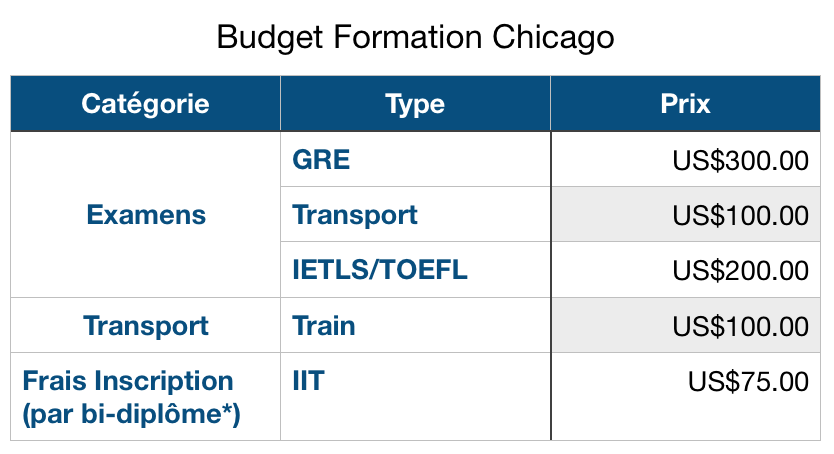
\includegraphics[width = 120mm]{figures/Budget_Chicago}
\caption{Indicatif de prix pour les tests à passer}
\end{figure}


\section{La timeline de formation}\label{sec:sec2.5}

\begin{figure}[h!]
\centering
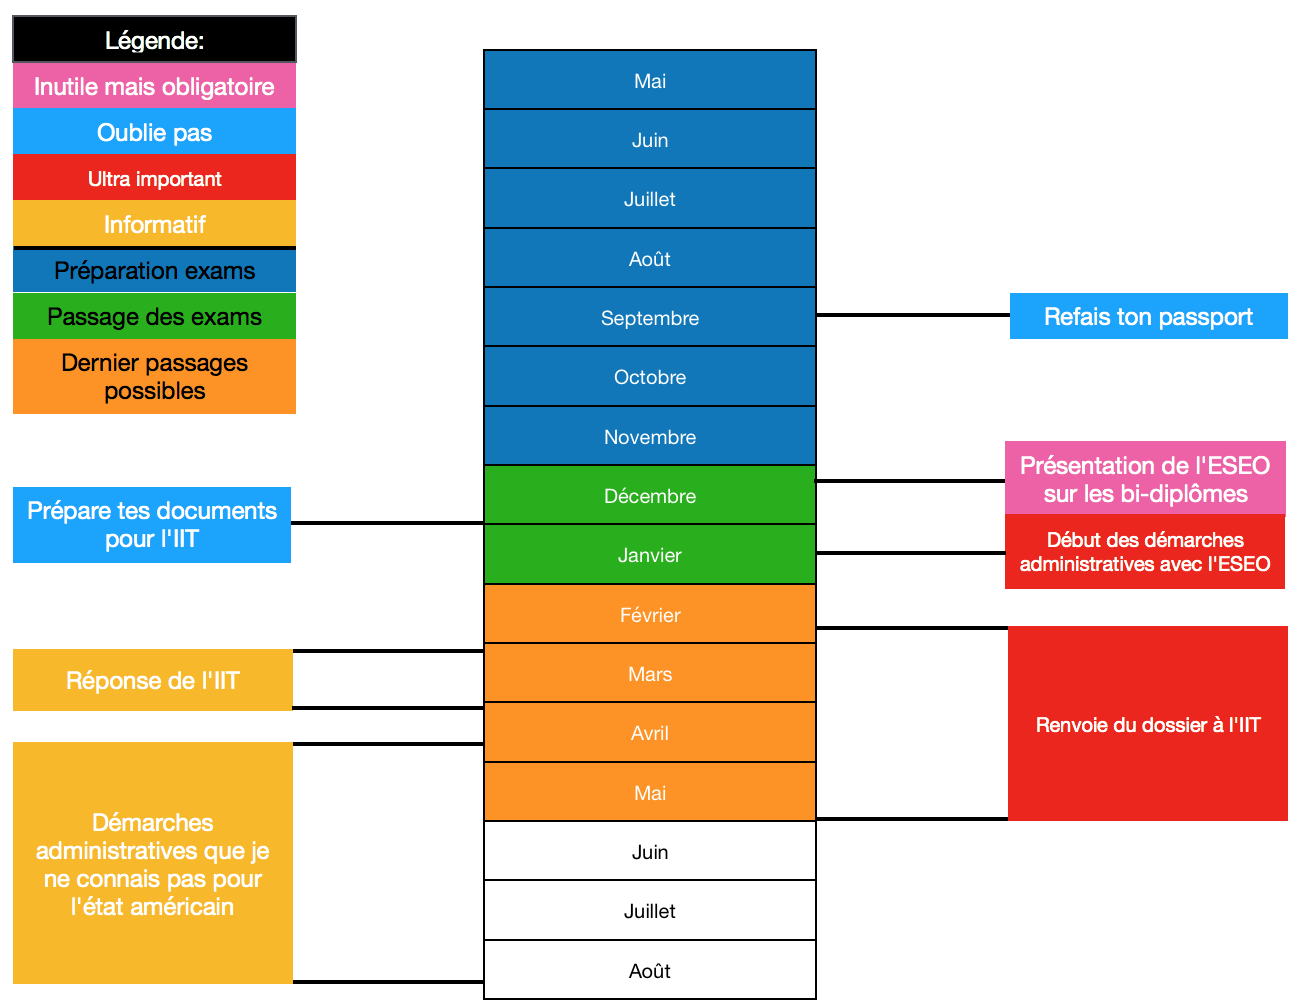
\includegraphics[width = 140mm]{figures/Chrono_Chicago}
\caption{Timeline indicative des deadlines}
\end{figure}
